\documentclass{article}

\usepackage{amsmath, amsthm, amssymb, amsfonts}
\usepackage{thmtools}
\usepackage{graphicx}
\usepackage{setspace}
\usepackage{geometry}
\usepackage{float}
\usepackage[utf8]{inputenc}
\usepackage[english]{babel}
\usepackage{framed}
\usepackage[dvipsnames]{xcolor}
\usepackage{tcolorbox}
\usepackage{hyperref}

\colorlet{LightGray}{White!90!Periwinkle}
\colorlet{LightOrange}{Orange!15}
\colorlet{LightGreen}{Green!15}

\theoremstyle{plain}% default
\newtheorem{thm}{Theorem}[section]
\newtheorem{lem}[thm]{Lemma}
\newtheorem{prop}[thm]{Proposition}
\newtheorem{prcp}[thm]{Principle}
\newtheorem*{cor}{Corollary}
\newtheorem*{KL}{Klein’s Lemma}

\theoremstyle{definition}
\newtheorem{defn}{Definition}[section]
\newtheorem{exmp}{Example}[section]
\newtheorem{xca}[exmp]{Exercise}
\theoremstyle{remark}
\newtheorem*{rem}{Remark}
\newtheorem*{note}{Note}
\newtheorem{case}{Case}

\newcommand{\HRule}[1]{\rule{\linewidth}{#1}}

% \declaretheoremstyle[name=Theorem,]{thmsty}
% \declaretheorem[style=thmsty,numberwithin=section]{theorem}
% \tcolorboxenvironment{theorem}{colback=LightGray}

% \declaretheoremstyle[name=Proposition,]{prosty}
% \declaretheorem[style=prosty,numberlike=theorem]{proposition}
% \tcolorboxenvironment{proposition}{colback=LightOrange}

% \declaretheoremstyle[name=Principle,]{prcpsty}
% \declaretheorem[style=prcpsty,numberlike=theorem]{principle}
% \tcolorboxenvironment{principle}{colback=LightGreen}

% \declaretheoremstyle[name=Definition,]{defsty}
% \declaretheorem[style=defsty,numberlike=theorem]{defn}
% \tcolorboxenvironment{defn}{colback=White}

\setstretch{1.2}
\geometry{
	textheight=9in,
	textwidth=5.5in,
	top=1in,
	headheight=12pt,
	headsep=25pt,
	footskip=30pt
}

% ------------------------------------------------------------------------------

\begin{document}
	
	% ------------------------------------------------------------------------------
	% Cover Page and ToC
	% ------------------------------------------------------------------------------
	
	\title{ \normalsize \textsc{}
		\\ [2.0cm]
		\HRule{1.5pt} \\
		\LARGE \textbf{\uppercase{Discrete Mathematics}
			\HRule{2.0pt} \\ [0.6cm] \LARGE{A Lecture Note} \vspace*{10\baselineskip}}
	}
	\date{}
	\author{\textbf{Arseto Satriyo Nugroho} \\ 
		Lecturer \\
		Diponegoro University \\
		2024}
	
	\maketitle
	\newpage
	
	\tableofcontents
	\newpage
	
	% ------------------------------------------------------------------------------
	
	% \section{Sets}
	
	% \begin{thm}
	% 	This is a theorem.
	% \end{thm}
	
	% \begin{prop}
	% 	This is a proposition.
	% \end{prop}
	
	% \begin{prcp}
	% 	This is a principle.
	% \end{prcp}

	% \begin{defn}[About something]
	% 	THis is a definition about something
	% \end{defn}
	
	% Maybe I need to add one more part: Examples.
	% Set style and colour later.
	
	% \subsection{Pictures}

	% \begin{defn}[About something]
	% 	THis is a definition about something
	% \end{defn}
	
	% \begin{figure}[htbp]
	% 	\center
	% 	\includegraphics[scale=0.06]{img/photo.jpg}
	% 	\caption{Sydney, NSW}
	% \end{figure}
	
	% \subsection{Citation}
	
	% This is a citation\cite{Eg}.
	
	% \newpage

	% \section{Relations}

	% \newpage
	
	% \section{Functions}

	% \newpage

	% \section{Logic}

	% \newpage

	% \section{Combinatorics}

	% \newpage

	\section{Graph Theory}
	\subsection{Overview}
	Graph theory is the study of graphs, which are mathematical structures used to model pairwise relations between objects.
	Originated in the 18th century by Leonhard Euler to solve the famous Seven Bridges of Königsberg problem.
	Widely applicable in computer science, mathematics, sociology, biology, and many other fields.

	\subsection{Basic Definitions}

	\begin{defn}[Graph]
		A Graph G Consists of a set of vertices V and a set of edges E, where each edge connects two vertices.
	\end{defn}

	\begin{equation}\label{eq-graph}
		G = (V, E)
	\end{equation}

	\begin{equation}\label{eq-vertex}
		V=\{v_1, v_2, v_3, ..., v_n\}
	\end{equation}

	\begin{equation}\label{eq-edge}
		E=\{(v_1,v_2), (v_2,v_3), ... \}
	\end{equation}

	A graph is denoted by pair of vertices and edges as shown in \eqref{eq-graph}.
	With vertex set is represented as \eqref{eq-vertex}, and edge set is represented as \eqref{eq-edge}.

	\begin{defn}[Vertex]
		A vertex, or a node, represents an entity in a graph.
	\end{defn}

	\begin{defn}[Edge]
		An edge, or a link, represents connection between two vertices.
	\end{defn}

	\begin{figure}[htbp]
		\center
		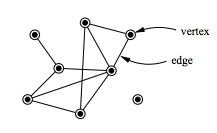
\includegraphics[scale=0.8]{img/graph-vertex-edge.png}
		\caption{Vertex and Edge}
	\end{figure}

	Notice that an edge connects exactly two vertices, and a vertex may be \textit{incident} to multiple edges.
	Two connected vertices are called \textit{adjacent} vertices.
	The number of edges incident to a vertex is called \textit{degree} of a vertex.


	\subsection{Graph Types}

	\subsubsection{Simple Graph, Multigraph, Pseudo Graph}

	Considering the pairing of the vertices, graph can be classified as simple graph
	(Figure \ref{fig-simple}), multigraph (Figure \ref{fig-multi}), and pseudograph (Figure \ref{fig-pseudo}).

	\begin{defn}[Simple Graph]
		A graph that doesn't contain any parallel edge nor loop.
	\end{defn}

	\begin{figure}[htbp]
		\center
		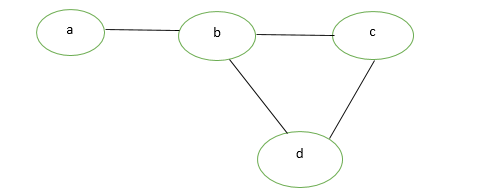
\includegraphics[scale=0.5]{img/simple-graph.png}
		\caption{Simple Graph}
		\label{fig-simple}
	\end{figure}

	\begin{defn}[Multi Graph]
		A graph that contains parallel edge but not self loop.
	\end{defn}

	\begin{defn}[Parallel Edge]
		If a pair of vertices connected by more than one edge.
	\end{defn}

	\begin{figure}[htbp]
		\center
		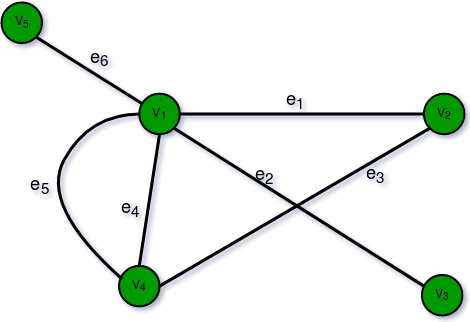
\includegraphics[scale=0.4]{img/multi-graph.png}
		\caption{Multi Graph}
		\label{fig-multi}
	\end{figure}

	\begin{defn}[Pseudo Graph]
		A multi graph that contains self loop.
	\end{defn}

	\begin{defn}[Self Loop]
		If an edge connects the same vertex.
	\end{defn}

	\begin{figure}[htbp]
		\center
		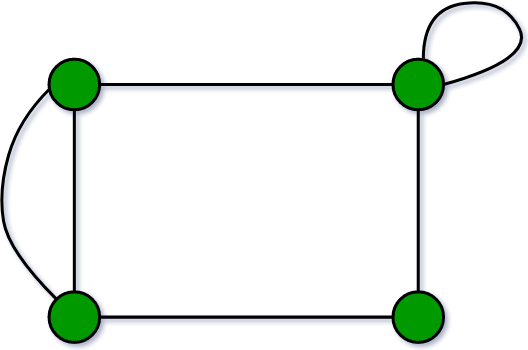
\includegraphics[scale=0.3]{img/pseudo-graph.png}
		\caption{Pseudo Graph}
		\label{fig-pseudo}
	\end{figure}


	\subsubsection{Undirected Graph vs Directed Graph}

	Graph can be either directed or undirected.
	A directed graph is indicated by arrow on the edges.
	In directed graph, traversal only allowed in the direction of the arrows.

	\begin{defn}[Undirected Graph]
		A graph in which edges have no direction.
	\end{defn}

	\begin{defn}[Directed Graph]
		A graph in which edges have direction.
	\end{defn}

	In undirected graph, $(u,v)$ is the same as $(v,u)$. But for directed graph, they are not the same, because the direction matters, $(u,v)$ means $u$ is the initial vertex $v$ is the terminal vertex.

	\subsubsection{Complete Graph}

	Complete graph is a graph that every vertex is adjacent to all other vertices. In other words, for a graph with $n$ vertex, every vertex has $n-1$ degree.

	\begin{figure}[htbp]
		\center
		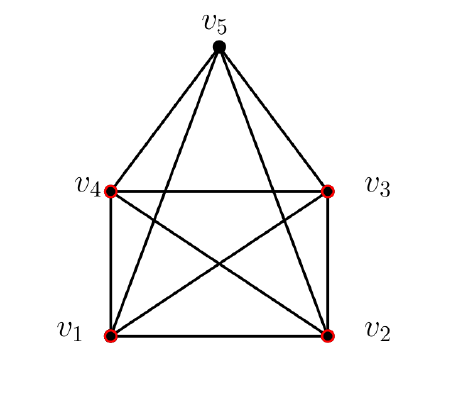
\includegraphics[scale=0.3]{img/complete-graph.png}
		\caption{Complete Graph}
		\label{fig-complete-graph}
	\end{figure}

	\subsubsection{Complement Graph}

	Complement of graph $G = (V, E)$ is graph $H$ with same vertices such that two vertices of $H$ are adjacent if and only if they are not adjacent in $G$. In other words, a complement graph of $G$ contains the same vertices and includes only missing edges of $G$ to form a complete graph. Hence the name 'complement'.

	\begin{figure}[htbp]
		\center
		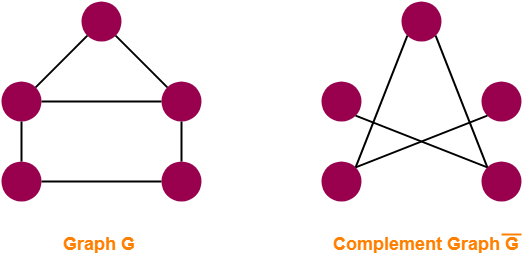
\includegraphics[scale=0.3]{img/complement-graph.png}
		\caption{Complement Graph}
		\label{fig-complement}
	\end{figure}

	\subsubsection{Bipartite Graph}

	Bipartite graph is with its vertices can be divided into two disjoint and independent sets $U$ and $V$, that is, every edge connects a vertex in $U$ to one in $V$, as shown in Figure \ref{fig-bipartite}. Equivalently, a bipartite graph is a graph that does not contain any odd-length cycles.

	\begin{figure}[htbp]
		\center
		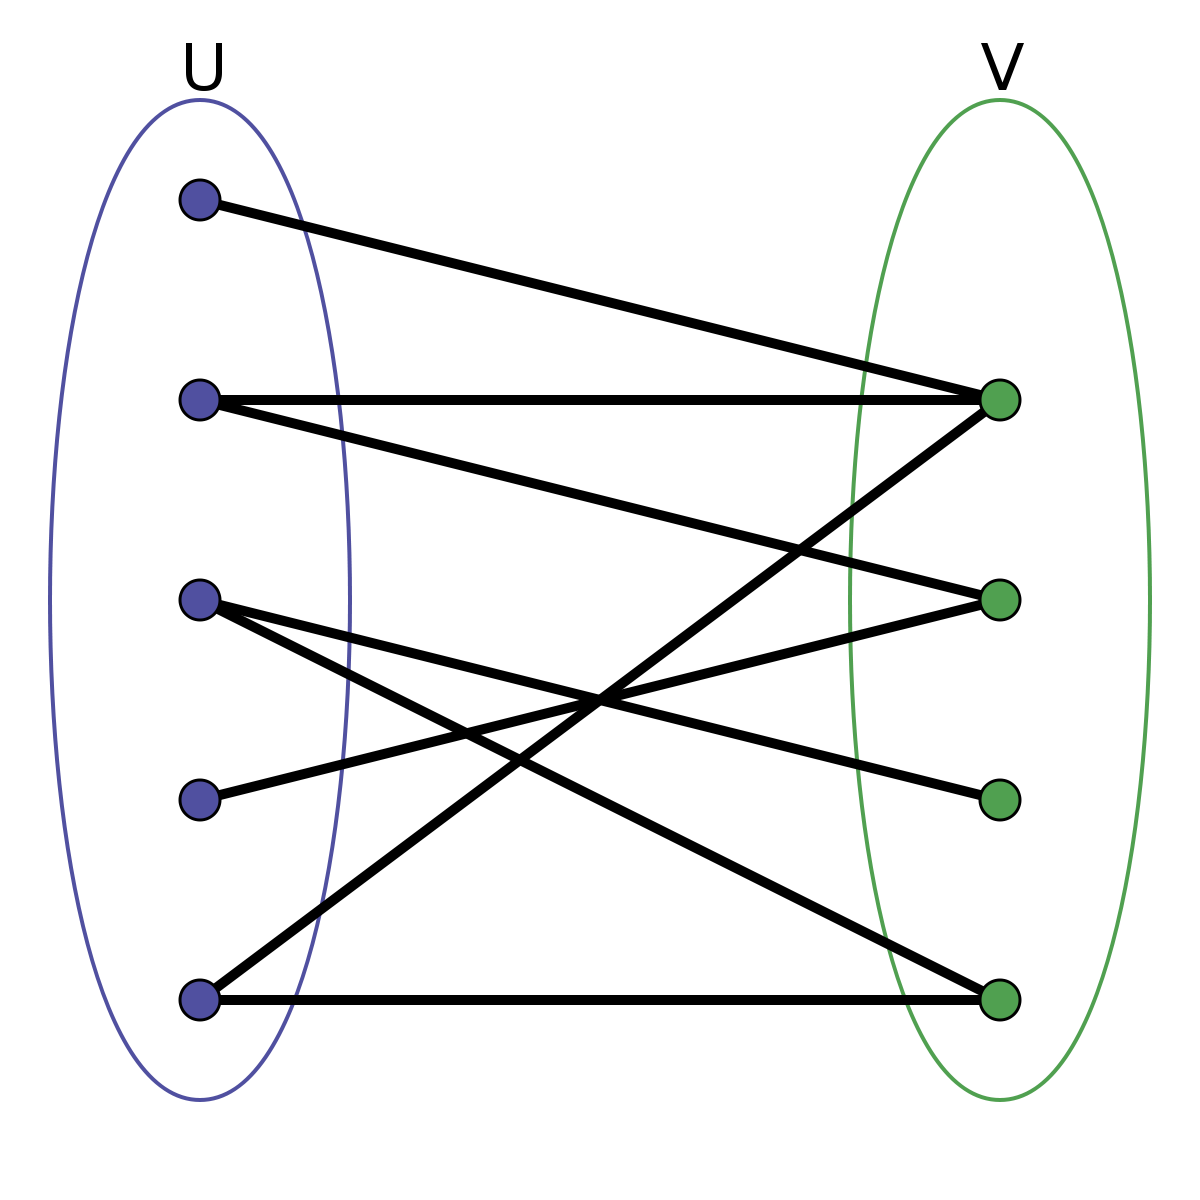
\includegraphics[scale=0.1]{img/bipartite-graph.png}
		\caption{Bipartite Graph}
		\label{fig-bipartite}
	\end{figure}

	A bipartite graph can be identified by (among other methods):
	\begin{enumerate}
		\item Choose any vertex in the graph for example, $x$.
		\item Assign it to one of the two sets, for this example, set to $U$ ($x$ is now an element of $U$).
		\item Assign all vertices adjacent to $x$ to the other set, for this example, $V$.
		\item For each vertex in $V$, assign all vertices adjacent to it to set $U$. And for each vertex in $U$, assign all vertices adjacent to it to set $V$.
		\item Repeat step 3 until all vertices have been assigned to a set.
		\item Check if any two adjacent vertices are in the same set. If yes, then the graph is not bipartite, otherwise it is bipartite.
	\end{enumerate}

	\subsubsection{Sub Graph}

	Graph $Gsub = (V_{sub}, E_{sub})$ is a sub graph of graph $G = (V, E)$ if $V_{sub} \in V$ and $E_{sub} \in E$

	\subsubsection{Connected Graph}

	A graph is connected if there exists a path from any vertex to any other vertex in the graph. In other words, all vertices at least adjacent to one other vertex.

	\subsection{Path and Circuit}

	\begin{defn}[Path]
		A path is a sequence of vertices with each vertex adjacent to the next one that starts and ends in different vertex and travels over any edge only once.
	\end{defn}

	\begin{defn}[Circuit]
		A circuit is a path that starts and ends at the same vertex.
	\end{defn}

	\subsubsection{Euler Circuit}

	\begin{defn}[Euler Path]
		A path that travels through every edge of a connected graph once and only once, and starts and ends at different vertices.
	\end{defn}

	For example, consider graph in Figure \ref{fig-graph-with-euler-path}. One of the euler path is F, A, B, C, F, E, C, D, E as shown in Figure \ref{fig-example-euler-path}.

	\begin{figure}[htbp]
		\center
		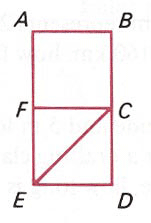
\includegraphics[scale=0.5]{img/euler-path-graph.png}
		\caption{Example Graph for Euler Path}
		\label{fig-graph-with-euler-path}
	\end{figure}

	\begin{figure}[htbp]
		\center
		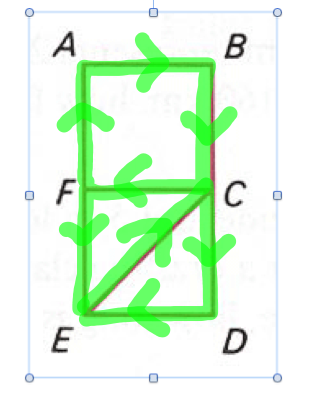
\includegraphics[scale=0.4]{img/euler-path.png}
		\caption{Example Euler Path}
		\label{fig-example-euler-path}
	\end{figure}

	\begin{defn}[Euler Circuit]
		An Euler Path that starts and ends at the same vertex.
	\end{defn}

	Consider a graph in Figure \ref{fig-graph-with-euler-circuit}. One euler circuit for the graph is E, A, B, F, E, F, D, C, E. Notice that it travels every edge once and only once, and starts and ends at the same vertex.

	\begin{figure}[htbp]
		\center
		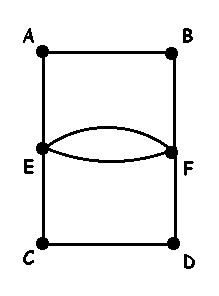
\includegraphics[scale=0.5]{img/euler-circuit-graph.png}
		\caption{Example Graph for Euler Circuit}
		\label{fig-graph-with-euler-circuit}
	\end{figure}

	\begin{figure}[htbp]
		\center
		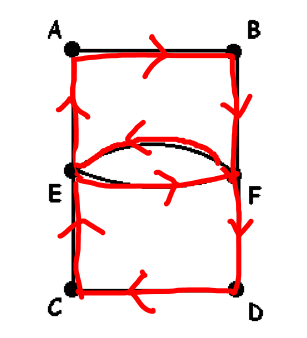
\includegraphics[scale=0.4]{img/euler-circuit.png}
		\caption{Example Euler Circuit}
		\label{fig-example-euler-circuit}
	\end{figure}

	\begin{thm}
		If a graph has any vertices of odd degree, then it cannot have an Euler Circuit.
	\end{thm}
	
	Equivalently, if a graph is connected and every vertex has an even degree, then it has at least one Euler circuit.

	\begin{thm}
		If a graph has more than two vertices of odd degree, then it cannot have an Euler path.
	\end{thm}

	Equivalently, a graph is connected and has exactly two vertices of odd degree 

	\subsection{Hamilton's Circuit}

	\begin{defn}[Hamilton Path]
		A path that must pass through each vertex of a graph once and only once.
	\end{defn}

	\begin{defn}[Hamilton Circuit]
		A circuit that must pass through each vertex of a graph once and only once.
	\end{defn}

	Notice that the main difference from Euler path/circuit is that hamilton path/circuit concerns vertex instead of edge.

	\begin{figure}[htbp]
		\center
		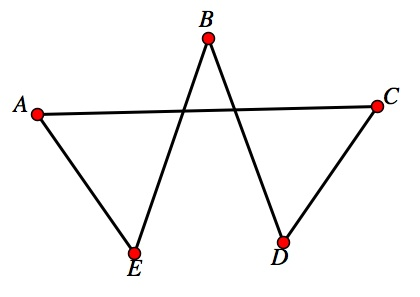
\includegraphics[scale=0.4]{img/hamilton-graph-a.png}
		\caption{Graph A}
		\label{fig-hamilton-graph-a}
	\end{figure}

	\begin{figure}[htbp]
		\center
		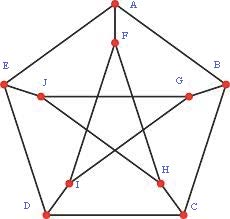
\includegraphics[scale=0.4]{img/hamilton-graph-b.png}
		\caption{Graph B}
		\label{fig-hamilton-graph-b}
	\end{figure}

	\begin{figure}[htbp]
		\center
		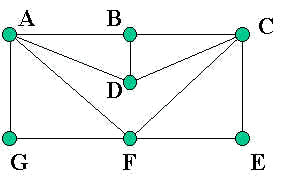
\includegraphics[scale=0.4]{img/hamilton-graph-c.png}
		\caption{Graph C}
		\label{fig-hamilton-graph-c}
	\end{figure}

	Not all graphs have hamilton circuit/path. There is no way to tell that the graph is hamiltonian using theorems like the case of euler path/circuit. Instead, we can do trial and error or devise an algorithm to do it. The case of hamiltonian circuit/path is used in Travelling Salesman Problem. See above graphs for examples.

	If a graph has a Hamilton circuit, then it has a Hamilton path, just stop before going back to the starting vertex. Graph A (Figure \ref{fig-hamilton-graph-a}) has a Hamilton circuit (one example:ACDBEA). Graph B (Figure \ref{fig-hamilton-graph-b}) has a hamilton path (one example: ABCDEJGIFH) but no hamilton circuit. And graph C (Figure \ref{fig-hamilton-graph-c}) has a hamilton circuit (one example: AGFECDBA).

	\subsection{Isomorphism}

	Unless the elements of the sets are labeled, we cannot distinguish amongst them. Given two graphs, $G$ and $H$ as in Figure \ref{fig-ex-isomorphism}.

	\begin{figure}[htbp]
		\center
		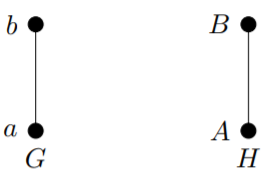
\includegraphics[scale=0.4]{img/isomorph-a.png}
		\caption{Example Isomorphism}
		\label{fig-ex-isomorphism}
	\end{figure}

	\begin{defn}[Isomorphism]
		Two graphs $G_1 = (V_1, E_1)$ and $G_2 = (V_2, E_2)$ are isomorphic if there is a bijection (a one-to-one, onto map) $\varphi$ from $V_1$ to $V_2$ such that:

		\begin{equation}\label{eq-isomorphism}
			\{v,w\} \in E_1 \Leftrightarrow \{\varphi(v),\varphi(w) \} \in E_2
		\end{equation}
	\end{defn}

	\begin{figure}[htbp]
		\center
		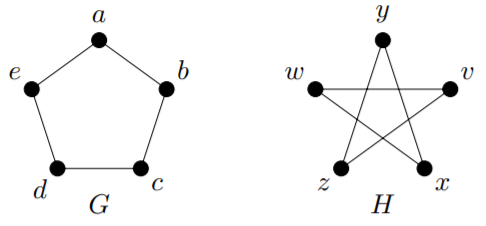
\includegraphics[scale=0.4]{img/isomorph-b.png}
		\caption{Example Isomorphism 5 vertex}
		\label{fig-ex-isomorphism-2}
	\end{figure}

	Graph $G$ and $H$ in Figure \ref{fig-ex-isomorphism-2}, the map $\varphi$ defined by:

	\begin{itemize}
		\item $\varphi (a) = v;$
		\item $\varphi (b) = z;$
		\item $\varphi (c) = y;$
		\item $\varphi (d) = x;$
		\item $\varphi (e) = w;$
	\end{itemize}

	Observe graph in Figure \ref{fig-ex-isomorphism-2}, notice that graph $G$ and $H$ fulfill the propositions below.

	\begin{prop}
			If graph $G_1$ and $G_2$ doesn't have same number of vertices, then they are not isomorphs.
	\end{prop}

	\begin{prop}
			If graph $G_1$ and $G_2$ doesn't have same number of edges, then they are not isomorphs.
	\end{prop}

	\begin{prop}
			If we list the degrees of vertices in $G_1$ and do the same for $G_2$, the lists will be the same but possibly in the different order.
	\end{prop}

	Using the same propositions, the graph below can be proofed not isomorphic, as they are not isomorphs according to the third proposition.

	\begin{figure}[htbp]
		\center
		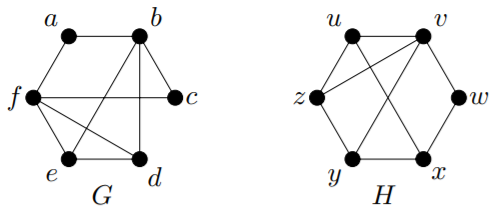
\includegraphics[scale=0.4]{img/graph-not-isomorphic-a.png}
		\caption{Example not isomorph}
		\label{fig-ex-isomorphism-3}
	\end{figure}

	Even so, being excluded from all those three propositions doesn't guarantee that the graphs are isomorphs. As in the case of graphs in Figure \ref{fig-ex-isomorphism-4}. Because although they are excluded from all three propositions above, if we observe closely we can see that in the second graph, the two vertices having same degree $\{f, c\}$ should be mapped to $\{z, v\}$. The vertex mapped to $u$ must be direct neighbors to the vertices having degree three, which are f and c. We can see that in the first graph, the the vertices having degree three doesn't have same neighbors.

	\begin{figure}[htbp]
		\center
		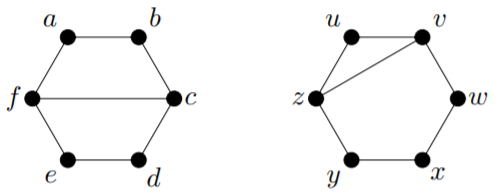
\includegraphics[scale=0.4]{img/graph-not-isomorphic-b.png}
		\caption{Example not isomorph (2)}
		\label{fig-ex-isomorphism-4}
	\end{figure}

	\subsection{Directed Graph}

	A graph in which the edges can only allow travel to one direction, it is called a directed graph, or digraph in short.

	\begin{defn}[Directed Graph]
		A directed graph consists of two sets, $V$ whose elements are the vertices of the digraph; and $E$ whose elements are ordered pairs from $V$ as in equation \ref{eq-directed-graph}. Elements of $E$ are referred as arc or directed edge, or simply edge.
	\end{defn}

	\begin{equation}\label{eq-directed-graph}
		A \subseteq \{ (v_1, v_2) | v_1, v_2 \in V\}
	\end{equation}

	\begin{figure}[htbp]
		\center
		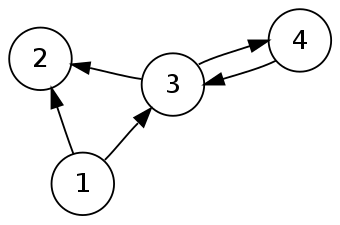
\includegraphics[scale=0.4]{img/directed-graph.png}
		\caption{Directed Graph}
		\label{fig-directed-graph}
	\end{figure}

	Example of directed graph representation shown at Figure \ref{fig-directed-graph}. Notice that the edge (directed edge) have arrows that indicates their direction. For example 3 - 2, is not equal with 2 - 3. If travel is permitted in both directions, it will have separate edges with opposing direction as in 3 - 4 and 4 - 3.

	The number of edges leaving a vertex is called out-degree. The number of edges entering a vertex is called in-degree.

	\subsubsection{Connectedness}

	A connected digraph can be divided into two categories: strongly connected or weakly connected. A digraph is called strongly connected if there exists path from any vertex to any other vertex as shown in Figure \ref{fig-strongly-connected}. In a weakly connected digraph, all vertices has edge entering or leaving it, but some vertices may not connected by path as shown in Figure \ref{fig-weakly-connected}.

	Notice that in Figure \ref{fig-weakly-connected}, vertex 1 cannot be reached from vertices 2,3, and 4. Whereas in Figure \ref{fig-strongly-connected} any vertex can be reached from any other vertex.

	\begin{figure}[htbp]
		\center
		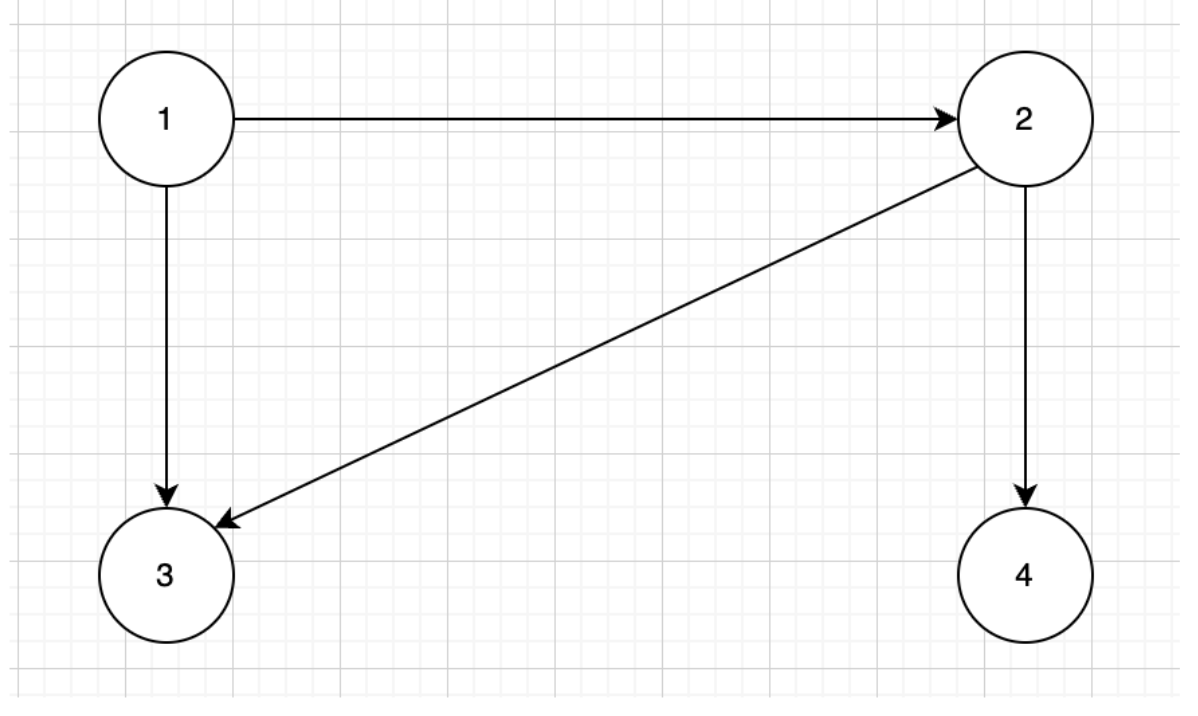
\includegraphics[scale=0.4]{img/weakly-connected.png}
		\caption{Weakly Connected Digraph}
		\label{fig-weakly-connected}
	\end{figure}

	\begin{figure}[htbp]
		\center
		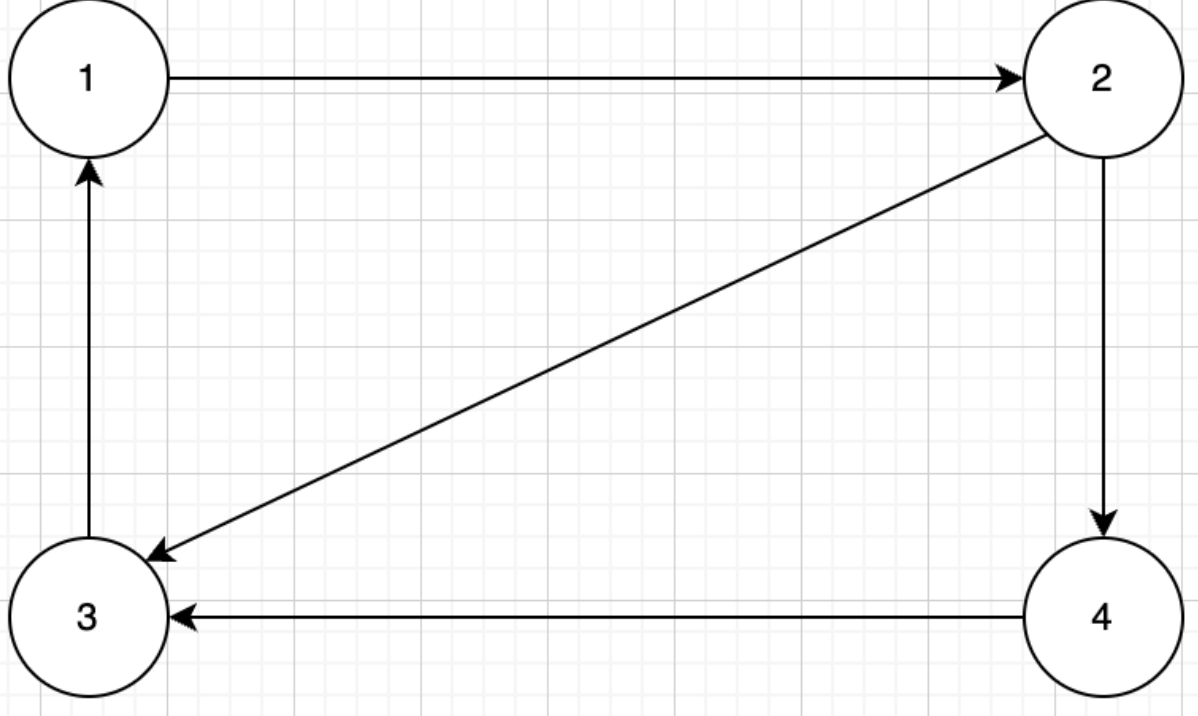
\includegraphics[scale=0.4]{img/strongly-connected.png}
		\caption{Strongly Connected Digraph}
		\label{fig-strongly-connected}
	\end{figure}

	\subsection{Matrix Representation}

	\subsubsection{Adjacency Matrix}

	\href{https://www.geeksforgeeks.org/graph-and-its-representations/}{Link to article}

	Important points:

	\begin{itemize}
		\item Both rows and columns represent vertices, so it will always be a square Matrix
		\item Undirected graph will have symmetrical matrix representation with diagonal as mirror
		\item Logically, ssymetrical matrix indicate directed graph
		\item Diagonal elements will always have 0 value in simple graph (as there is no loop)
	\end{itemize}

	\newpage
	
	% ------------------------------------------------------------------------------
	% Reference and Cited Works
	% ------------------------------------------------------------------------------
	
	% \bibliographystyle{IEEEtran}
	% \bibliography{References.bib}
	
	% ------------------------------------------------------------------------------
	
\end{document}
